% Chapter Template

\chapter{Historical background} % Main chapter title

\label{Chapter01} % Change X to a consecutive number; for referencing this chapter elsewhere, use \ref{ChapterX}



%----------------------------------------------------------------------------------------
%   SECTION 1
%----------------------------------------------------------------------------------------

\section{The human computer}

\begin{figure}[ht]
    \centering
    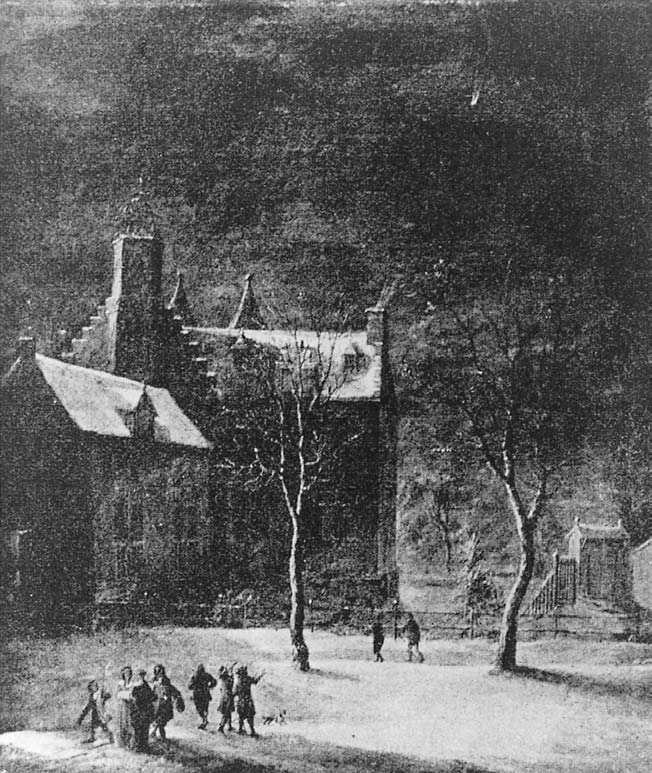
\includegraphics[width=0.75\textwidth]{comet}
    \caption{Halley's comet over Cambridge, 1682\cite{grier2010}}
    \label{fig:comet}
\end{figure}

In order to better understand the history of simulation, it is useful to take a look at the history of computation in general, and how the need to simulate and predict the behavior of physical systems
has been a driving force in the development of both analog and digital computers. While analog counting devices, such as the Chinese abacus, have been used for thousands of years to aid in
computation, the term originally applied to the profession. The beginnings of the profession can be traced to the work done by Alexis-Claude Clairaut to predict the perihelion, the closest approach to
the sun, of Halley's comet. While the return of the comet had been a matter of scientific discussion since it was first predicted by Edmund Halley in 1695, the period of time between earlier sightings
did not conform to Halley's prediction. The orbit calculated by Halley, using his own measurements from the 1682 passing, predicted that the comet would reappear at fixed intervals. However, the
appearances of the comet, recorded by Apian in 1531, Kepler in 1607, and Halley himself in 1682, did not conform to a perfectly regular interval. Halley and Newton correctly deduced that other
celestial bodies influenced the comet's orbit, but the three-body problem was considered insurmountable at the time. Beginning in the spring of 1757, one year before the predicted return of the comet,
Clairaut began to undertake the calculation of the comet's orbit, using differential equations solved by successive approximation\cite{wilson1993}. Clairaut set two friends to calculating the
positions of Jupiter and Saturn, around the sun, advancing them a degree or two for every step of the calculation, the computing the forces that acted on them and the effect on their orbits. Clairaut
calculated the resulting effect on the comet itself. They did these calculations, first starting with the 1531 return, and having done that repeated the work starting with the 1607 observations and
finally the 1682 observation by Halley, working daily from June through September of 1757. While the prediction produced by Clairaut's team would deviate from the date of the perihelion by 33 days, it
was a vast improvement compared to the prediction of Halley, which had an error margin of 600 days. Ultimately, while several shortcomings have later been identified in the calculations performed by
Clairaut, his largest contribution was not the prediction of Halley's comet itself, but the idea that laborious mathematics could be computed in parallel; that mathematical work could be divided into
pieces, computed independently, checked for errors and combined into a final product\cite{grier2010}.

Shortly after the work by Clairaut and his companions, the French Académie des Sciences undertook to calculate logarithmic and trigonometric tables for the new metric system. Inspired by Adam Smith's
writings on division of labor in the Wealth of Nations, Gaspard de Prony, director of the Bureau du Cadastre, organized the bureau's computing staff into three sections. The first group was made up of
workers without training in mathematics, who would perform simple arithmetics. The second group, made up of more experienced computers, reduced the calculations that were to be performed into
fundamental arithmetical operations, and verified the results that were returned. These made up the section that in later computing organizations would be referred to as planners. The operation was
overseen by some of the finest mathematicians in France. This section took no part in the computational work itself, but investigated the various analytical expressions that could be used, and
selected the ones best suited for reduction into simple steps\cite{hyman1985}.

%----------------------------------------------------------------------------------------
%   SECTION 2
%----------------------------------------------------------------------------------------

\section{Analog computers}

\begin{figure}[ht]
    \centering
    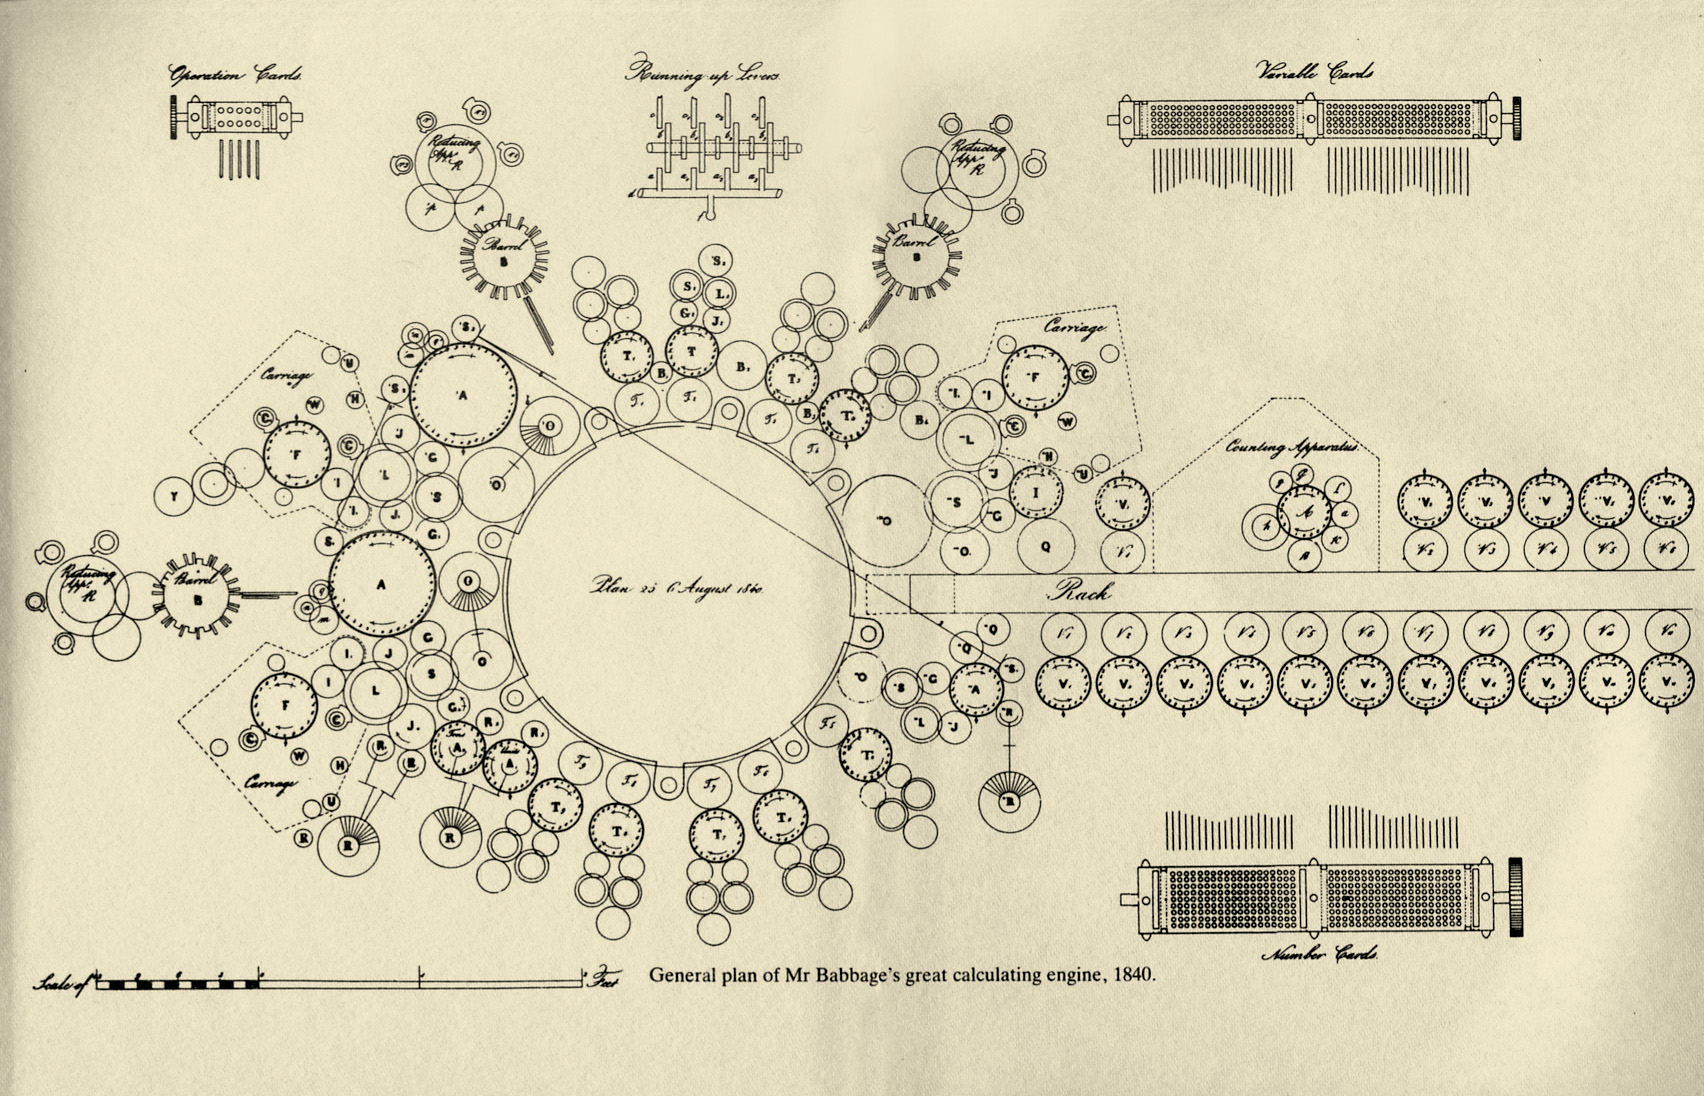
\includegraphics[width=0.\textwidth]{engine}
    \caption{Babbage's Analytical Engine\cite{diffengine}}
    \label{fig:engine}
\end{figure}

Working with a similar project in 1821, Charles Babbage, widely considered the father of the computer, was familiar with the approach used by de Prony and applied a similar methodology. Like de Prony,
Babbage recognized that mathematical work could be reduced to what he called mental labor\cite{babbage1832}. He applied the same approach as de Prony in calculating a series of tables for the
Astronomical Society of London. However, Babbage was disappointed by the number of mistakes done by the human computers in his employ. Babbage took de Prony's approach to its next logical step and
began work on a calculating machine. Applying the finite difference method, Babbage designed his first difference engine: an analog computer that could calculate the values of a polynomial simply by
using repeated addition.

While the difference engine designed by Babbage holds great historical interest, the Astronomical Society which supported its creation ultimately did not adopt it for
practical use, as it was cumbersome in operation. Instead, the first machines to gain widespread acceptance among astronomical computers would be the geared adding machine. The geared adding machine
was invented in the 17th century, but it would only be with the aid of 19th century mass production menthods, and the consequent reduction in their cost, that the machines would proliferate.

Human computers did not do the were employed by mathematicians to perform calculations, such as processing data. These men and women weren't doing the creative tasks of mathematicians, but
were rather doing work that Charles Babbage referred to as "mental labor"\cite{babbage1832}. While the computation of large amounts of data was central to several important projects before the 18th
century, the history of organized computing arguably begins

Before the ubiquitousness of the modern, digital computer, the term would refer to the profession, namely a person who would perform
calculation. This use of the term dates back several hundred years.

The first machine we recognize as a computer today was designed by Babbage i 1839. Working with Ada Countess Lovelace, widely considered the first programmer

The term "computer", meaning the profession, dates back to the 17th century. Research laboratories, such as those operated by the Manhattan Project, and later by the National Advisory Committee for
Aeronautics (the precursor to NASA), established computing sections in order to perform calculations more efficiently than engineers could do themselves. These computers did a wide variety of work in
nuclear physics, flight research and later the early space program \cite{mclennan2012computer}.

While simple analog computers like the slide rule had been in use for several hundred years, the need to perform complex calculations during the war drove the development of increasingly complex
analog computers, such as Marchant desktop calculators, and IBM punched-card machines\cite{carr}, to the invention of the digital computer.

One of the first digital computers, along with the Colossus used for cryptanalysis at Bletchley Park\cite{sep-computing-history}, was the ENIAC. The machine was brought online on February 14, 1946
at the University of Pennsylvania, where it had been built by a team led by John Mauchly and J. Presper Eckert, at the Moore School of Electrical Engineering. The computer was originally designed to
calculate artillery firing tables for the military. Though far from general purpose, its design was sufficiently flexible to allow calculations to solve a wide variety of numerical problems
\cite{10.2307/2002620}. The ENIAC was quickly put to use solving other problems, and one of the first real-world applications for the machine was the work on nuclear fusion by Edward Teller
\cite{AtomicHeritageFoundation}.

The ideas developed by the people who had worked on the ENIAC, and its successor the EDVAC, were disseminated in 1946 at the Moore School Lectures. Scientists at the Moore School had already begun
work on the EDVAC, which would be the first binary computer, and the school was central to many of the earliest developments in digital computing. The attendees at the lectures were all established
academics, physicists and mathematicians and the lectures led to an explosion of activity in both the United States and Europe \cite{Davis2008}.

The research in nuclear physics started during the war continued in peacetime and scientists at the Los Alamos National Laboratory had a large backlog of computing needs. There was a desire to apply
statistical methods, among them the Monte Carlo method, to solve some of these problems, including calculations to find deeply neutrons would permeate various materials. This had previously been done
by large numbers of human computers. The Monte Carlo method uses statistical sampling to allow for the simulation of problems that can't be solved otherwise, but is very time consuming to do by hand.
To alleviate this, researchers wished to use the new digital computer to do the calculations \cite{Haigh2014}. However, the ENIAC was designed as a large collection of functional modules, and was
programmed by manually connecting these to one another with a large switchboard. This meant that while the computer was very fast by the standards at the time, setting the machine up to solve a new
problem could take weeks \cite{Rope2007}. In 1948, a new control system was planned and implemented for the ENIAC. The new system, based on the work of John von Neumann \cite{VonNeumann1993}
\cite{Haigh2014a} added an instruction set to the computer, which greatly simplified its operation, and arguably gave birth to the first stored-program computer \cite{Rope2007}. In this way, the need
to quickly simulate a wide variety of mathematical problems directly led to the creation of the modern general-purpose computer.

%-----------------------------------
%   SUBSECTION 1
%-----------------------------------

\subsection{Subsection 1}
Nunc posuere quam at lectus tristique eu ultrices augue venenatis. Vestibulum ante ipsum primis in faucibus orci luctus et ultrices posuere cubilia Curae; Aliquam erat volutpat. Vivamus sodales tortor eget quam adipiscing in vulputate ante ullamcorper. Sed eros ante, lacinia et sollicitudin et, aliquam sit amet augue. In hac habitasse platea dictumst.

%-----------------------------------
%   SUBSECTION 2
%-----------------------------------

\subsection{Subsection 2}
Morbi rutrum odio eget arcu adipiscing sodales. Aenean et purus a est pulvinar pellentesque. Cras in elit neque, quis varius elit. Phasellus fringilla, nibh eu tempus venenatis, dolor elit posuere quam, quis adipiscing urna leo nec orci. Sed nec nulla auctor odio aliquet consequat. Ut nec nulla in ante ullamcorper aliquam at sed dolor. Phasellus fermentum magna in augue gravida cursus. Cras sed pretium lorem. Pellentesque eget ornare odio. Proin accumsan, massa viverra cursus pharetra, ipsum nisi lobortis velit, a malesuada dolor lorem eu neque.

%----------------------------------------------------------------------------------------
%   SECTION 2
%----------------------------------------------------------------------------------------

\section{The dawn of the digital computer}

\begin{figure}[ht]
    \centering
    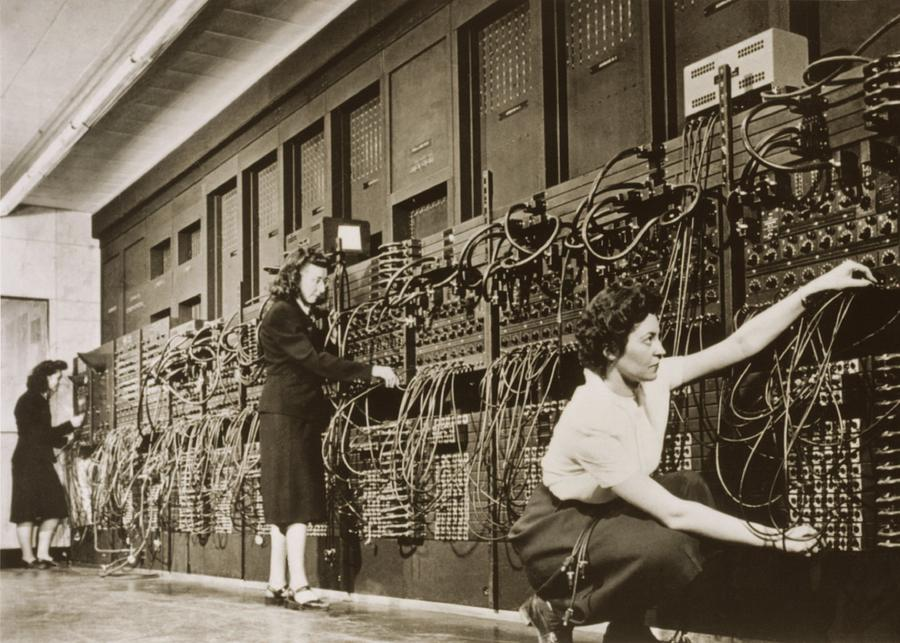
\includegraphics[width=0.75\textwidth]{eniac}
    \caption{Technicians programming the ENIAC \cite{LosAlamosNationalLaboratory}}
    \label{fig:eniac}
\end{figure}

Sed ullamcorper quam eu nisl interdum at interdum enim egestas. Aliquam placerat justo sed lectus lobortis ut porta nisl porttitor. Vestibulum mi dolor, lacinia molestie gravida at, tempus vitae ligula. Donec eget quam sapien, in viverra eros. Donec pellentesque justo a massa fringilla non vestibulum metus vestibulum. Vestibulum in orci quis felis tempor lacinia. Vivamus ornare ultrices facilisis. Ut hendrerit volutpat vulputate. Morbi condimentum venenatis augue, id porta ipsum vulputate in. Curabitur luctus tempus justo. Vestibulum risus lectus, adipiscing nec condimentum quis, condimentum nec nisl. Aliquam dictum sagittis velit sed iaculis. Morbi tristique augue sit amet nulla pulvinar id facilisis ligula mollis. Nam elit libero, tincidunt ut aliquam at, molestie in quam. Aenean rhoncus vehicula hendrerit.
